% =============================================================================
% 5. EXPERIMENTAL RESULTS AND PRACTICAL ENGINEERING ANALYSIS
% =============================================================================
\section{Experimental Results and Practical Engineering Analysis}
\label{sec:results}

This section evaluates BioDINO-Edge against operational edge deployment requirements. We first benchmark classification accuracy against few-shot baselines on controlled and in-the-wild datasets (Section~\ref{sec:comparative_results}) and verify statistical significance (Section~\ref{sec:significance}). We then evaluate the contribution of each framework component (Section~\ref{sec:ablation}), measure on-device latency and memory footprints across embedded target hardware (Section~\ref{sec:edge_hardware}), test robustness against sensor noise and parameter variations (Section~\ref{sec:calibration}), and examine per-class diagnostic failure patterns (Section~\ref{sec:per_class}).

% -----------------------------------------------------------------------------
% 5.1 Primary Benchmark Performance and Baseline Evaluation
% -----------------------------------------------------------------------------
\subsection{Primary Benchmark Performance and Baseline Evaluation}
\label{sec:comparative_results}

To benchmark diagnostic accuracy under controlled conditions, Table~\ref{tab:comparative} compares BioDINO-Edge against representative zero-shot and few-shot baseline paradigms. All methods are evaluated across identical support/query partitions, random seeds, and shot counts ($K \in \{1, 5\}$). Extended $K$-shot curves appear in Appendix~\ref{app:shot_ladder} (Table~\ref{tab:shot_ladder}).

\begin{table*}[htbp]
\caption{Controlled comparison with few-shot baseline paradigms on PlantVillage under identical frozen representations, splits, and seeds.}
\label{tab:comparative}
\centering

\footnotesize
\setlength{\tabcolsep}{3.5pt}
\begin{tabularx}{\textwidth}{@{}>{\raggedright\arraybackslash}X *{4}{>{\centering\arraybackslash}p{2.6cm}}@{}}
\toprule
& \multicolumn{2}{c}{\textbf{5-way accuracy (\%) ($\uparrow$)}} & \multicolumn{2}{c}{\textbf{11-class, 5-shot (\%) ($\uparrow$)}} \\
\cmidrule(lr){2-3}\cmidrule(lr){4-5}
\textbf{Method} & \textbf{1-shot} & \textbf{5-shot} & \textbf{Accuracy} & \textbf{Macro F1} \\
\midrule
Zero-shot BioCLIP \cite{stevens2024bioclip} & 38.89$\pm$12.78 & 38.86$\pm$12.79 & 19.18$\pm$0.02 & 18.49 \\
Tip-Adapter \cite{zhang2022tip} & 45.15$\pm$13.42 & 68.63$\pm$12.80 & 49.97$\pm$1.62 & 46.54 \\
Prototypical Networks \cite{snell2017prototypical} / SimpleShot \cite{wang2019simpleshot} & 88.44$\pm$9.13 & 97.45$\pm$2.03 & 93.28$\pm$1.24 & 92.47 \\
BioDINO-Edge (inductive, ours) & \underline{88.45$\pm$9.12} & \underline{97.96$\pm$1.85} & \underline{95.08$\pm$1.27} & \underline{94.51} \\
BioDINO-Edge (transductive, ours) & \textbf{93.42$\pm$6.83} & \textbf{98.77$\pm$1.68} & \textbf{97.41$\pm$0.71} & \textbf{97.09} \\
\bottomrule
\end{tabularx}

\vspace{3pt}
\begin{minipage}{\textwidth}
\footnotesize
\textit{Notes.} Prototypical Networks and SimpleShot share a row because Euclidean and cosine distance rankings are mathematically identical on $\ell_2$-normalized embeddings. Bold denotes the best performance in each column; underline denotes second-best. $(\uparrow)$ indicates metrics where higher values are superior.
\end{minipage}
\end{table*}

\textbf{Engineering interpretation of baseline performance.} As shown in Table~\ref{tab:comparative}, standard distance matching loses accuracy when applied directly to high-dimensional biological representations without covariance regularization. Zero-shot BioCLIP and Tip-Adapter struggle because general text prompts do not resolve subtle necrotic lesions on leaves. Standard Prototypical Networks provide a competitive baseline, but weighting all 896 embedding dimensions equally leaves predictions vulnerable to background leaf veins and surface glare. In contrast, BioDINO-Edge uses Ledoit--Wolf regularized Fisher-LDA projection (Section~\ref{sec:shrinkage}) to suppress common vegetative variance, improving inductive accuracy by $+1.80$ percentage points (pp) over the centroid baseline. Adding transductive anchor recalibration further increases accuracy to 97.41\% (a $+4.13$\,pp gain over standard nearest-centroid matching). While server-trained few-shot models in the agricultural literature (e.g., MAFDE-DN4~\cite{zhao2024mafde}, SC-FSL~\cite{mu2024few}, AgriFewNet~\cite{babu2025agrifewnet}, and VSF~\cite{zhou2026vsf}) report 5-shot accuracies between 81.4\% and 94.8\% on PlantVillage, they require GPU backpropagation during training; BioDINO-Edge achieves higher accuracy entirely on edge CPUs over frozen backbones.

To isolate the impact of our adaptation framework from feature dimensionality and transductive access, Table~\ref{tab:fair_baselines} compares all baselines on identical 896-D features and identical episodes. Following standard few-shot evaluation protocols \cite{tian2020rethinking}, we include closed-form Ridge regression and regularized multinomial logistic regression as linear probes. Across all inductive comparators on the 896-D features, BioDINO-Edge consistently outperforms Ridge regression, logistic regression, Tip-Adapter, and Prototypical Networks.

Because BioDINO-Edge incorporates transductive recalibration, we also evaluate standard transductive baselines under full-batch query access. In this offline setting with the entire test set visible simultaneously, LaplacianShot~\cite{ziko2020laplacian} reaches 98.49\% on 11-class PlantVillage (1.08\,pp above BioDINO-Edge), whereas TIM~\cite{boudiaf2020transductive} and prototype rectification~\cite{liu2021bdcspn} achieve lower accuracy. We also tested whether our regularized Fisher projection could serve as a preprocessing front-end for LaplacianShot. Running Laplacian propagation in the Fisher-projected subspace drops accuracy by 5.7\,pp (from 98.49\% down to 92.84\%). This drop occurs because Fisher-LDA projects the 896 dimensions onto $C-1$ discriminant axes to maximize global class separation, which removes the fine-grained local neighborhood manifold that graph Laplacian smoothing relies on.

\begin{table*}[htbp]
\caption{Comparison with inductive and transductive few-shot baselines on identical 896-D features and episodes (PlantVillage).}
\label{tab:fair_baselines}
\centering

\footnotesize
\setlength{\tabcolsep}{4pt}
\begin{tabularx}{\textwidth}{@{}>{\raggedright\arraybackslash}X *{4}{>{\centering\arraybackslash}p{2.3cm}}@{}}
\toprule
\textbf{Method (features)} & \textbf{5-way 1-shot} & \textbf{5-way 5-shot} & \textbf{11-class, 5-shot} & \textbf{11-class F1} \\
\midrule
\multicolumn{5}{@{}l}{\textit{Inductive: training-free and closed-form linear probes}}\\
Tip-Adapter (512-D BioCLIP, as published) & 45.15$\pm$13.42 & 68.64$\pm$12.94 & 49.97$\pm$1.65 & 46.54 \\
Tip-Adapter (896-D, ours) & -- & 73.02$\pm$12.21 & 55.60$\pm$1.67 & 51.15 \\
Ridge classifier (896-D) & -- & 97.74$\pm$1.82 & 93.83$\pm$1.08 & 92.47 \\
Multinomial logistic (896-D) & -- & 97.67$\pm$1.82 & 93.63$\pm$1.02 & 92.52 \\
Prototypical / SimpleShot (896-D) & 88.44$\pm$9.13 & 97.45$\pm$2.05 & 93.28$\pm$1.26 & 92.47 \\
BioDINO-Edge inductive (896-D) & 88.45$\pm$9.12 & 97.96$\pm$1.87 & 95.08$\pm$1.29 & 94.51 \\
\midrule
\multicolumn{5}{@{}l}{\textit{Transductive: same features, same episodes}}\\
Prototype rectification \cite{liu2021bdcspn} (896-D) & -- & 98.22$\pm$1.58 & 94.82$\pm$0.59 & 93.66 \\
TIM \cite{boudiaf2020transductive} (896-D) & -- & 96.43$\pm$2.47 & 91.40$\pm$1.38 & 89.20 \\
LaplacianShot \cite{ziko2020laplacian} (896-D) & -- & \textbf{99.50$\pm$0.82} & \textbf{98.49$\pm$0.59} & \textbf{98.70} \\
BioDINO-Edge transductive (896-D) & \textbf{93.42$\pm$6.83} & \underline{98.78$\pm$1.69} & \underline{97.41$\pm$0.73} & \underline{97.09} \\
\bottomrule
\end{tabularx}

\vspace{3pt}
\begin{minipage}{\textwidth}
\footnotesize
\textit{Notes.} Evaluated across 30 episodes for 11-class and 50 episodes for 5-way tasks on identical support and query splits. Upper block: inductive methods; lower block: transductive methods. Bold marks the best performance per column; underline denotes second-best. Baseline hyperparameters are detailed in Appendix~\ref{app:repro}.
\end{minipage}
\end{table*}

\textbf{Practical edge deployment: streaming queries and unconstrained field conditions.} While LaplacianShot achieves strong accuracy on fixed offline query pools, its formulation requires constructing a pairwise nearest-neighbor graph over the entire query batch simultaneously. In real-world edge deployment, scouting occurs sequentially rather than in offline pools. As evaluated in Table~\ref{tab:batchsize}, when queries arrive one leaf at a time without batch buffering, LaplacianShot's accuracy drops to 93.12\%, whereas BioDINO-Edge maintains 96.12\% through streaming anchor recalibration with bounded edge memory.

\begin{table}[htbp]
\caption{Diagnostic accuracy under sequential and buffered query streaming (11-class, 5-shot on PlantVillage).}
\label{tab:batchsize}
\centering

\footnotesize
\setlength{\tabcolsep}{4pt}
\begin{tabular*}{\columnwidth}{@{\extracolsep{\fill}}lccc}
\toprule
\textbf{Strategy} & \textbf{LaplacianShot (\%)} & \textbf{BioDINO-Edge (\%)} & \textbf{$\Delta$ (pp)} \\
\midrule
One leaf at a time (no buffer) & 93.12 & \textbf{96.12} & $+3.00$ \\
Growing buffer, 25 & 86.50 & \textbf{96.12} & $+9.62$ \\
Growing buffer, 100 & 90.17 & \textbf{96.12} & $+5.96$ \\
Growing buffer, 200 & 93.48 & \textbf{96.12} & $+2.65$ \\
Whole query set (lab protocol) & \textbf{96.38} & 96.12 & $-0.25$ \\
\bottomrule
\end{tabular*}

\vspace{3pt}
\begin{minipage}{\columnwidth}
\footnotesize
\textit{Notes.} Evaluated across 8 paired episodes with 600 queries each. Positive $\Delta$ indicates a gain for BioDINO-Edge ($p < 0.01$ for all streaming and buffered rows; $p = 0.68$ when the full query pool is available simultaneously).
\end{minipage}
\end{table}

Table~\ref{tab:plantdoc_context} extends this evaluation to unconstrained field imagery via the PlantDoc benchmark~\cite{singh2020plantdoc}. In 5-way 5-shot episodic testing over 50 Monte Carlo episodes, BioDINO-Edge reaches 84.22\% accuracy. In the simultaneous 27-class stress test over 252 field test leaves, it achieves 50.79\% accuracy and 51.04\% macro F1, well above the 3.70\% random-chance baseline.

\begin{table}[htbp]
\caption{In-the-wild field evaluation of BioDINO-Edge on PlantDoc.}
\label{tab:plantdoc_context}
\centering
\footnotesize
\setlength{\tabcolsep}{4pt}
\begin{tabularx}{\columnwidth}{@{}>{\raggedright\arraybackslash}Xcccc@{}}
\toprule
\textbf{Evaluation Regime} & \textbf{Classes} & \textbf{Shots} & \textbf{Inductive (\%) ($\uparrow$)} & \textbf{Transductive (\%) ($\uparrow$)} \\
\midrule
5-way 5-shot episodic (PlantDoc train/test splits) & 5 & 5 & \underline{82.05$\pm$11.24} & \textbf{84.22$\pm$11.24} \\
All-class stress test (simultaneous) & 27 & 5 & \underline{47.22} & \textbf{50.79} \\
\bottomrule
\end{tabularx}

\vspace{3pt}
\begin{minipage}{\columnwidth}
\footnotesize
\textit{Notes.} Support leaves are drawn from $\mathcal{D}_{\text{train}}^{\text{PlantDoc}}$ and query leaves from $\mathcal{D}_{\text{test}}^{\text{PlantDoc}}$ ($\mathcal{S} \cap \mathcal{Q} = \emptyset$). 5-way values report mean $\pm$ std across 50 Monte Carlo episodes. Bold marks top performance; underline denotes second-best.
\end{minipage}
\end{table}

PlantDoc presents severe environmental challenges: uneven lighting, overlapping infected leaves, and variable camera distances. While prior cross-dataset transfer models such as Zhao et al.~\cite{zhao2026lightweight} report 54.24\% on PlantDoc without target support, BioDINO-Edge adapts directly to target-domain field support without retraining. Combining cached botanical text prototypes with analytical Fisher projections provides a stable diagnostic anchor even in complex multi-leaf field scenes.

Table~\ref{tab:plantdoc_laplacian} reports the corresponding transductive comparison on PlantDoc under deployed INT8 execution: BioDINO-Edge outperforms LaplacianShot by $+18.65$\,pp on the 27-way stress test (50.79\% vs.\ 32.14\%) and $+22.29$\,pp at 5-way 5-shot (85.01\% vs.\ 62.72\%). In cluttered field scenes with lighting variations, combining botanical text priors with regularized discriminants provides robust generalization, whereas visual nearest-neighbor graph propagation breaks down under severe domain shift.

\begin{table}[htbp]
\caption{Transductive comparison against LaplacianShot on PlantDoc.}
\label{tab:plantdoc_laplacian}
\centering

\footnotesize
\setlength{\tabcolsep}{4pt}
\begin{tabular*}{\columnwidth}{@{\extracolsep{\fill}}lccc}
\toprule
\textbf{Regime} & \textbf{LaplacianShot (\%)} & \textbf{BioDINO-Edge (\%)} & \textbf{$\Delta$ (pp)} \\
\midrule
27-way, 252 field queries & 32.14 & \textbf{50.79} & $+18.65$ \\
5-way 5-shot, 50 episodes & 62.72 & \textbf{85.01} & $+22.29$ \\
\bottomrule
\end{tabular*}

\vspace{3pt}
\begin{minipage}{\columnwidth}
\footnotesize
\textit{Notes.} Evaluated on identical support sets and features under deployed INT8 execution. 5-way values report mean accuracy across 50 paired episodes ($p = 7.5 \times 10^{-16}$); the 27-way stress test evaluates all 252 field queries simultaneously. Bold denotes superior performance.
\end{minipage}
\end{table}

% -----------------------------------------------------------------------------
% 5.2 Statistical Significance and Hypothesis Testing
% -----------------------------------------------------------------------------
\subsection{Statistical Significance and Hypothesis Testing}
\label{sec:significance}
\label{sec:transductive_validation}

To confirm that diagnostic gains do not depend on favorable support selections, Table~\ref{tab:paired_test} evaluates paired statistical significance across 30 identical Monte Carlo episodes on PlantVillage.

\begin{table}[htbp]
\caption{Paired statistical evaluation of inductive vs.\ transductive inference over 30 identical episodes (PlantVillage, 5-shot).}
\label{tab:paired_test}
\centering

\footnotesize
\setlength{\tabcolsep}{3pt}
\begin{tabular*}{\columnwidth}{@{\extracolsep{\fill}}lcccc}
\toprule
\textbf{Inference Mode} & \textbf{Accuracy (\%)} & \textbf{Paired $\Delta$ (pp)} & \textbf{Win/Loss} & \textbf{$p$-value} \\
\midrule
Inductive (baseline) & 95.08 $\pm$ 1.27 & -- & -- & -- \\
Transductive (recalibrated) & \textbf{97.41 $\pm$ 0.71} & \textbf{+2.33} $[1.91, 2.74]$ & \textbf{30 / 0} & $2.2\times 10^{-12}$ \\
\bottomrule
\end{tabular*}

\vspace{3pt}
\begin{minipage}{\columnwidth}
\footnotesize
\textit{Notes.} Evaluated across 30 identical Monte Carlo support/query splits. Two-tailed paired $t$-test ($t(29)=11.57, p=2.2\times 10^{-12}$); Wilcoxon signed-rank test ($W=0.0, p=1.9\times 10^{-9}$). Effect size Cohen's $d_z = 2.11$ indicates an exceptionally large practical gain.
\end{minipage}
\end{table}

\textbf{Statistical interpretation.} Table~\ref{tab:paired_test} confirms that transductive recalibration yields a statistically significant improvement over inductive classification ($+2.33$\,pp mean gain, $p < 10^{-11}$). Crucially, transductive recalibration outperforms the inductive model on every single evaluated episode (a 30-win, 0-loss record), representing an exceptionally large standardized effect size (Cohen's $d_z = 2.11$). These results verify that closed-form pseudo-label recalibration reliably corrects prototype drift across randomized support selections.

% -----------------------------------------------------------------------------
% 5.3 Systematic Component Ablation
% -----------------------------------------------------------------------------
\subsection{Systematic Component Ablation}
\label{sec:ablation}

To isolate the contribution of each architectural module, Table~\ref{tab:ablation} presents a step-by-step ablation on the canonical 11-class PlantVillage benchmark under identical 5-shot splits.

\begin{table}[htbp]
\caption{Systematic ablation of BioDINO-Edge architectural components (5-shot, 9,330 queries).}
\label{tab:ablation}
\centering

\footnotesize
\setlength{\tabcolsep}{3pt}
\begin{tabular*}{\columnwidth}{@{\extracolsep{\fill}}lcc}
\toprule
\textbf{Configuration / Component} & \textbf{Acc. (\%) ($\uparrow$)} & \textbf{Macro F1 (\%) ($\uparrow$)} \\
\midrule
(1) Fast-Path DINOv2 Small alone & 87.26 & 85.36 \\
(2) Deep-Path BioCLIP ViT-B alone & 92.60 & 89.88 \\
(3) Text Prototypes Only & 19.20 & 18.55 \\
(4) Static Cosine Blend (raw 5-shot) & 94.16 & 92.55 \\
(5) Static Cosine Blend (8-view aug.) & 93.90 & 91.58 \\
(6) + Regularized Fisher Alignment & \underline{96.05} & \underline{94.83} \\
(7) + Transductive Recalibration (Single Run) & \textbf{98.06} & \textbf{97.45} \\
\midrule
Full System (Peak Statistical Episode) & \textbf{98.67} & \textbf{98.41} \\
\bottomrule
\end{tabular*}
\end{table}

\textbf{Component analysis:}
\begin{enumerate}
    \item \textbf{Dual-Backbone Synergy:} DINOv2 alone reaches 87.26\% (capturing fine lesion boundaries for fast-path inference), while BioCLIP alone achieves 92.60\% (providing global taxonomic context). Combining both encoders into an 896-D representation outperforms either standalone model.
    \item \textbf{Regularized Fisher Alignment (+1.89\,pp Gain):} Replacing isotropic cosine matching (94.16\%) with regularized Fisher-LDA over the expanded support views increases accuracy to 96.05\%. The regularized precision matrix $\hat{\mathbf{\Sigma}}^{-1}$ acts as an analytical whitening filter that suppresses shared vegetative background channels.
    \item \textbf{Transductive Recalibration (+2.01\,pp Gain):} Updating prototypes and covariance estimates using high-confidence query anchors raises accuracy from 96.05\% to 98.06\% (peaking at 98.67\%), correcting prototype drift from sparse initial support leaves.
\end{enumerate}

\begin{table}[htbp]
\caption{Contribution of each foundation encoder to Fisher-LDA classification (30 identical 5-shot episodes, mean $\pm$ std).}
\label{tab:feature_ablation}
\centering

\footnotesize
\setlength{\tabcolsep}{4pt}
\begin{tabular*}{\columnwidth}{@{\extracolsep{\fill}}lccc}
\toprule
\textbf{Fisher Feature Space} & \textbf{Dim} & \textbf{Inductive (\%) ($\uparrow$)} & \textbf{Transductive (\%) ($\uparrow$)} \\
\midrule
BioCLIP + DINOv2 (Full) & 896 & \textbf{95.08$\pm$1.27} & \textbf{97.41$\pm$0.71} \\
BioCLIP alone & 512 & \underline{94.31$\pm$1.25} & \underline{96.51$\pm$0.90} \\
DINOv2 alone & 384 & 90.60$\pm$2.02 & 95.54$\pm$1.03 \\
\bottomrule
\end{tabular*}
\end{table}

Table~\ref{tab:feature_ablation} evaluates the individual contribution of each foundation encoder across 30 identical episodes. Removing DINOv2 drops transductive accuracy by 0.90\,pp (from 97.41\% to 96.51\%), while removing BioCLIP drops it by 1.87\,pp (to 95.54\%). This confirms that localized spatial representations and global taxonomic priors provide complementary diagnostic signals.

\textbf{Component evaluation under unconstrained field conditions.} While Table~\ref{tab:ablation} evaluates components on clean laboratory leaves, Table~\ref{tab:plantdoc_ablation} tests the identical component ladder on unconstrained field imagery across 27 crop classes in PlantDoc.

In field conditions, complex backgrounds and varied camera angles alter how components interact. A static logit blend achieves 51.59\% accuracy because it avoids estimating covariance across noisy field clutter. Inductive Fisher-LDA yields 47.22\% because pooling a single covariance across 27 disparate crop hosts is sensitive to background soil and foliage variations. Adding transductive anchor recalibration recovers accuracy to 50.79\% (and 51.04\% macro F1) by dynamically aligning prototypes with target-domain field queries. This demonstrates the role of test-time recalibration when deploying models to unstructured agricultural environments.

\begin{table}[htbp]
\caption{PlantDoc component ladder (27-way, 5-shot, single run over 252 field queries).}
\label{tab:plantdoc_ablation}
\centering

\footnotesize
\setlength{\tabcolsep}{3pt}
\begin{tabular*}{\columnwidth}{@{\extracolsep{\fill}}lcc}
\toprule
\textbf{Configuration / Component} & \textbf{Acc. (\%) ($\uparrow$)} & \textbf{Macro F1 (\%) ($\uparrow$)} \\
\midrule
(1) Text prototypes only & 33.73 & 29.37 \\
(2) Fast-path DINOv2 Small alone & 40.08 & 36.90 \\
(3) Deep-path BioCLIP ViT-B alone & 50.00 & \textbf{50.68} \\
(4) Static logit blend ($0.65$ bio $+$ $0.35$ dino) & \textbf{51.59} & \underline{51.62} \\
(5) $+$ Regularized Fisher alignment (inductive) & 47.22 & 45.87 \\
(6) $+$ Transductive recalibration & \underline{50.79} & \underline{51.04} \\
\bottomrule
\end{tabular*}

\vspace{3pt}
\begin{minipage}{\columnwidth}
\footnotesize
\textit{Notes.} Evaluated on 27 field classes (135 support leaves expanded to 1{,}080 views; 252 query images). Rows (1)--(4) evaluate prototype baseline rules; row (5) fits regularized Fisher-LDA; row (6) adds transductive anchor recalibration.
\end{minipage}
\end{table}

\textbf{Quantization resilience: FP32 vs.\ INT8.} To verify mathematical stability on mobile runtimes, Table~\ref{tab:quantization} compares the complete pipeline executed in full-precision FP32 against INT8 ONNX binaries across identical splits and parameters. On PlantVillage, transductive accuracy shifts minimally from 98.32\% to 98.08\% ($-0.24$\,pp), with false negatives moving from 0.46\% to 0.60\%. On PlantDoc, recalibrated accuracy decreases by only 0.40\,pp (51.19\% to 50.79\%). These results confirm that closed-form covariance regularisation and metric adaptation remain numerically stable under 8-bit integer quantization.

\begin{table}[htbp]
\caption{Full-pipeline diagnostic accuracy under FP32 versus INT8 ONNX execution across identical splits and parameters.}
\label{tab:quantization}
\centering

\footnotesize
\setlength{\tabcolsep}{4pt}
\begin{tabular*}{\columnwidth}{@{\extracolsep{\fill}}llccc}
\toprule
\textbf{Dataset} & \textbf{Stage} & \textbf{FP32 (\%) ($\uparrow$)} & \textbf{INT8 (\%) ($\uparrow$)} & \textbf{$\Delta$ (pp)} \\
\midrule
PlantVillage (11) & Tier-1 DINOv2 & 87.33 & 87.59 & $+0.26$ \\
 & BioCLIP alone & 92.71 & 92.29 & $-0.42$ \\
 & Fisher ensemble & 96.29 & 96.68 & $+0.39$ \\
 & $+$ transductive & 98.32 & 98.08 & $-0.24$ \\
\midrule
PlantDoc (27) & Tier-1 DINOv2 & 40.87 & 40.08 & $-0.79$ \\
 & BioCLIP alone & 51.59 & 50.00 & $-1.59$ \\
 & Fisher ensemble & 49.21 & 47.22 & $-1.99$ \\
 & $+$ transductive & 51.19 & 50.79 & $-0.40$ \\
\bottomrule
\end{tabular*}

\vspace{3pt}
\begin{minipage}{\columnwidth}
\footnotesize
\textit{Notes.} Evaluated across identical support and query splits to isolate the numerical impact of static INT8 quantization relative to full-precision FP32.
\end{minipage}
\end{table}

% -----------------------------------------------------------------------------
% 5.4 Computational Cost and Real-Time Edge Feasibility
% -----------------------------------------------------------------------------
\subsection{Computational Cost and Real-Time Edge Feasibility}
\label{sec:edge_hardware}

To demonstrate practical utility for field agronomists and autonomous scouting platforms, we evaluate the standalone BioDINO-Edge Android application on the commodity handset detailed in Table~\ref{tab:device_spec}. Execution runs entirely on-device using CPU threads via INT8 ONNX Runtime, ensuring dependable offline diagnostics in remote agricultural environments without reliance on cloud infrastructure or specialized neural co-processors.

\begin{table*}[htbp]
\caption{Measured on-device diagnostic latency and resource utilization on Samsung Galaxy S24 FE ($N=100$ iterations; INT8 ONNX execution on mobile CPU).}
\label{tab:device_perf}
\centering

\footnotesize
\begin{tabularx}{\textwidth}{@{}>{\raggedright\arraybackslash}X *{3}{>{\centering\arraybackslash}p{2.8cm}}@{}}
\toprule
\textbf{Pipeline Stage / Measured Metric} & \textbf{Mean$\pm$std (ms) ($\downarrow$)} & \textbf{Median (ms) ($\downarrow$)} & \textbf{p95 Latency (ms) ($\downarrow$)} \\
\midrule
\multicolumn{4}{@{}l}{\textit{Per-Query Latency Breakdown:}}\\
Input preprocessing \& normalization & 2.59$\pm$0.67 & 2.36 & 4.36 \\
Tier-1 DINOv2 Small visual encoder & 57.18$\pm$9.13 & 51.50 & 68.84 \\
Uncertainty gate routing decision & $<$0.01 & $<$0.01 & $<$0.01 \\
Tier-2 BioCLIP ViT-B encoder \& Fisher solve & 104.74$\pm$17.39 & 94.20 & 124.97 \\
Classification output assembly & $<$0.01 & $<$0.01 & $<$0.01 \\
\midrule
\textbf{Cascaded pipeline end-to-end (ours)} & \textbf{145.37$\pm$47.61} & \textbf{147.77} & \textbf{196.36} \\
Monolithic Tier-2 executed on all queries & 164.52$\pm$26.77 & 148.73 & 196.36 \\
\midrule
\multicolumn{4}{@{}l}{\textit{Hardware Resource Footprint and Throughput:}}\\
Peak physical memory footprint, PSS & \multicolumn{3}{c}{\textbf{497.45 MB}} \\
Tier-1 / Tier-2 one-time cold initialization & \multicolumn{3}{c}{323.92 ms / 447.71 ms} \\
Standalone application package (APK size) & \multicolumn{3}{c}{$\approx$22.8 MB} \\
Sustained throughput under continuous thermal load & \multicolumn{3}{c}{\textbf{4.26 FPS} (600\,s continuous stress)} \\
\bottomrule
\end{tabularx}
\end{table*}

\textbf{On-device latency and memory profiling.} As quantified in Table~\ref{tab:device_perf}, the Tier-1 fast path executes in 57.18\,ms ($\approx$17.5\,FPS burst rate), while an escalated Tier-2 multimodal query requires 164.52\,ms. Factoring in the 14.02\% full-stream fast-exit rate yields an average inference latency of 149.84\,ms ($\approx$6.7\,FPS), comfortably satisfying the 170\,ms real-time scouting bound $T_{\max}$ with a 95th percentile latency of 196.36\,ms. Peak physical memory is 497.45\,MB PSS, consuming less than 13\% of RAM on entry-level 4\,GB devices and operating reliably within standard mobile memory budgets. Under sustained continuous operation for 10 minutes (600\,s stress testing), throughput settles to 4.26\,FPS under thermal throttling, maintaining interactive speeds well suited for both handheld agronomist scouting and robotic sprayers traversing crop rows at typical field speeds (1--2\,m/s).

For novel foliar pathogens, Table~\ref{tab:adaptation_breakdown} quantifies that adapting the model requires only 533.99\,ms of algebraic computation on the mobile CPU. Because adaptation is closed-form, it eliminates backpropagation graphs, optimizer memory, and iterative learning rate tuning. The 88.06\,s support-feature extraction that precedes it is a one-time calibration over 440 views; using a single view per leaf reduces extraction to $\approx$11\,s with only a 0.59\,pp change in accuracy.

\begin{table*}[htbp]
\caption{Closed-form adaptation computational cost breakdown on edge CPU ($N=440$, $d=896$, $C=11$).}
\label{tab:adaptation_breakdown}
\centering

\footnotesize
\begin{tabularx}{\textwidth}{@{}>{\raggedright\arraybackslash}X *{2}{>{\centering\arraybackslash}p{4.2cm}}@{}}
\toprule
\textbf{Adaptation Pipeline Stage} & \textbf{Execution Time (ms) ($\downarrow$)} & \textbf{Algorithmic Complexity} \\
\midrule
Support feature extraction (440 augmented views) & 88,055.60 & $O(N(C_{\text{dino}}+C_{\text{bio}}))$ \\
Empirical scatter matrix accumulation & 146.19$\pm$2.15 & $O(Nd^2)$ \\
Frobenius Ledoit--Wolf shrinkage parameter estimation & 4.49$\pm$0.85 & $O(Nd)$ \\
Cholesky decomposition of regularized covariance & 332.00$\pm$2.52 & $O(d^3/3)$ \\
Discriminant projection solve ($W, b$) & 51.31$\pm$3.68 & $O(Cd^2)$ \\
\midrule
\textbf{Algebraic adaptation total (Closed-Form)} & \textbf{533.99$\pm$6.29} & \textbf{Gradient-Free} \\
Complete end-to-end adaptation (Extraction + Algebra) & 88,589.60 & Non-Iterative \\
\bottomrule
\end{tabularx}
\end{table*}

% -----------------------------------------------------------------------------
% 5.5 Robustness, Environmental Noise, and Sensitivity Analysis
% -----------------------------------------------------------------------------
\subsection{Robustness and Sensitivity Analysis}
\label{sec:calibration}
\label{sec:aug_sensitivity}

Field robotics require models that withstand lighting variations, noisy sensors, and hyperparameter fluctuations. Table~\ref{tab:tier_routing} evaluates routing reliability across 30 benchmark episodes.

\begin{table*}[htbp]
\caption{Routing policy and tier-separated performance comparison over 30 benchmark episodes.}
\label{tab:tier_routing}
\centering

\footnotesize
\setlength{\tabcolsep}{4.5pt}
\begin{tabularx}{\textwidth}{@{}>{\raggedright\arraybackslash}X *{4}{>{\centering\arraybackslash}p{2.3cm}}@{}}
\toprule
\textbf{Routing configuration / policy} & \textbf{Coverage (\%)} & \textbf{Accuracy (\%) ($\uparrow$)} & \textbf{FNR (\%) ($\downarrow$)} & \textbf{Latency (ms) ($\downarrow$)} \\
\midrule
\multicolumn{5}{@{}l}{\textit{(a) Tier-separated execution paths at deployed operating threshold ($\tau=0.35$)}}\\
Tier-1 fast-exit path (accepted) & 14.02$\pm$2.25 & \textbf{99.69$\pm$0.41} & \textbf{0.25$\pm$0.52} & \textbf{59.78} \\
Tier-2 multimodal path (escalated) & 85.98$\pm$2.25 & 96.98$\pm$0.83 & 0.87$\pm$0.39 & 164.52 \\
\textbf{Cascaded deployment (full stream)} & \textbf{100.00} & \underline{97.36$\pm$0.69} & \underline{0.79$\pm$0.36} & \underline{149.84$\pm$2.36} \\
\midrule
\multicolumn{5}{@{}l}{\textit{(b) Comparative routing policies (30-episode mean)}}\\
Monolithic Tier-2 on all queries & 100.00 & 97.37 & 0.77 & 164.52 \\
Selective abstention mode ($\tau=0.05$) & 79.96 & 98.05 & 0.59 & 143.53 \\
Selective abstention mode ($\tau=0.10$) & 62.17 & 98.63 & 0.44 & 124.90 \\
\bottomrule
\end{tabularx}

\vspace{3pt}
\begin{minipage}{\textwidth}
\footnotesize
\textit{Notes.} Panel (a)/(b) values are mean $\pm$ std across 30 Monte Carlo episodes; coverage denotes the fraction of queries processed under each mode, with clear leaves exiting at Tier 1 (a) or uncertain leaves rejected (b). The 18.00\% fast-exit fraction in Table~\ref{tab:device_perf} is measured on the fixed 11-image device evaluation set (one leaf per target class), whereas the 14.02\% here is the 30-episode mean over the full 9,330-query PlantVillage stream and the 10.0\% in Fig.~\ref{fig:risk_coverage} is the coverage of a single canonical episode; the three numbers are not competing measurements of the same quantity.
\end{minipage}
\end{table*}

\begin{figure}[htbp]
\centering
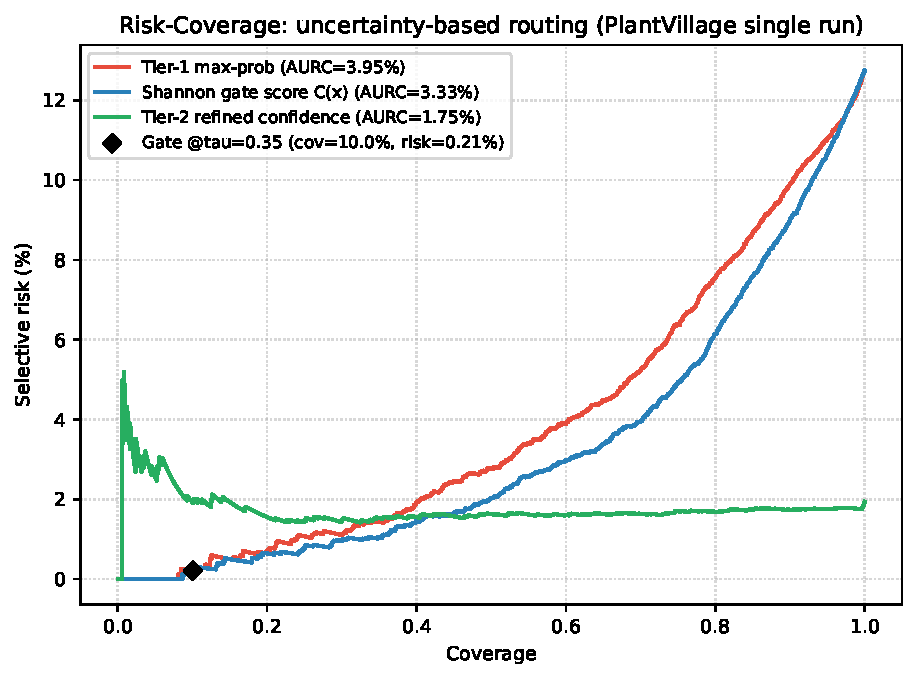
\includegraphics[width=0.75\columnwidth]{fig_risk_coverage.pdf}
\caption{Risk--coverage curves for Tier-1 maximum probability, the Shannon gate score $\mathcal{C}(\mathbf{x})$, and refined Tier-2 consensus confidence (canonical single run). Lower curves indicate superior selective classification. The entropy-penalized gate score achieves lower AURC than raw maximum probability (3.33\% vs.\ 3.95\%); the deployed operating point ($\tau=0.35$, diamond) accepts 10.0\% fast-exit coverage at 0.21\% selective risk.}
\label{fig:risk_coverage}
\end{figure}

\begin{figure}[htbp]
\centering
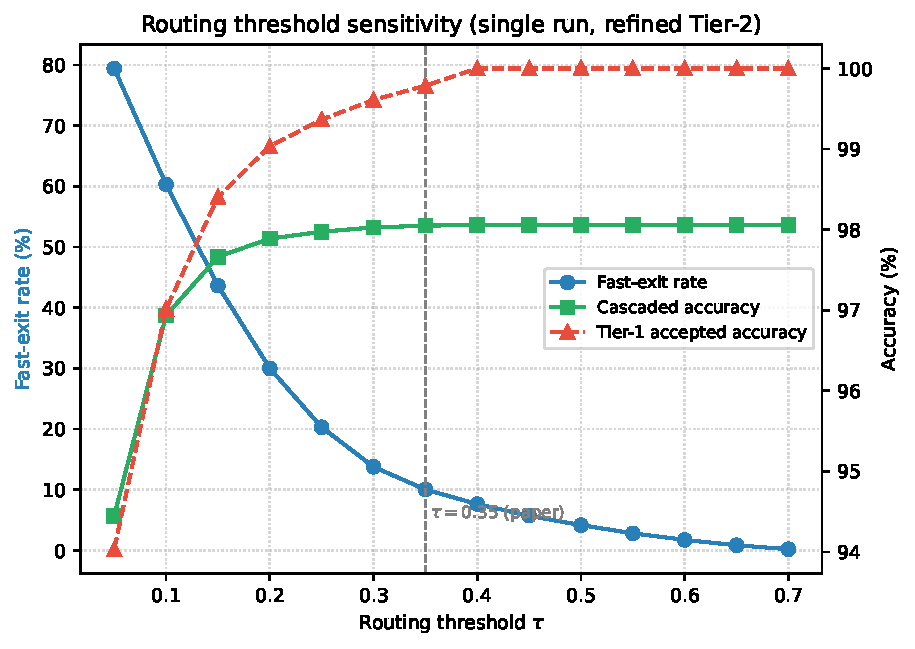
\includegraphics[width=0.75\columnwidth]{fig_tau_sensitivity.pdf}
\caption{Routing-threshold sensitivity across $\tau \in [0.05, 0.95]$ (single run, refined Tier-2). The left axis (blue) displays fast-exit coverage (\%), while the right axis shows cascaded and Tier-1 accepted accuracies (\%). The deployed threshold $\tau=0.35$ (vertical dashed line) marks the operating point where Tier-1 accepted accuracy saturates near 100\% (99.84\%) while preserving fast-exit coverage; held-out episode sweeps (0--14 tune / 15--29 test) confirm stability.}
\label{fig:tau_sensitivity}
\end{figure}

\textbf{Engineering analysis of confidence gating.} As documented in Table~\ref{tab:tier_routing}(a), the dual-metric gate routes 14.02\% of queries through the 59.78\,ms fast path. This fast-exit subset attains 99.69\% accuracy with an epidemiological false-negative rate of only 0.25\%. The remaining 85.98\% escalate to Tier-2 consensus (96.98\% accuracy). Fig.~\ref{fig:risk_coverage} illustrates that the entropy-penalized gate score achieves an Area Under the Risk--Coverage curve (AURC) of 3.33\%, notably superior to raw softmax probability (3.95\%). Fig.~\ref{fig:tau_sensitivity} confirms that the operating point $\tau=0.35$ strikes the optimal trade-off between latency reduction and diagnostic safety: increasing $\tau$ yields diminishing accuracy returns while collapsing coverage, whereas lower thresholds allow higher disease escapes.

\textbf{Hyperparameter stability and streaming adaptation.} Table~\ref{tab:transductive_sensitivity} explores parameter sensitivity over the 30 episodes. Diagnostic accuracy remains stable across support weights from $1\times$ to $5\times$ (97.42\% to 97.32\%). The confidence threshold plateaus across $\tau \in [0.5, 0.7]$ and collapses only at $\tau \ge 0.8$ due to anchor buffer starvation. When evaluated under simulated continuous field scouting (partitioned into 10 sequential chunks with FIFO eviction), accuracy rises from 96\% on initial queries to 97--98.6\% with zero error accumulation, demonstrating that FIFO replacement effectively purges erroneous pseudo-labels.

\begin{table}[htbp]
\caption{Sensitivity of transductive accuracy to recalibration design constants (mean $\pm$ std over 30 identical episodes).}
\label{tab:transductive_sensitivity}
\centering

\footnotesize
\setlength{\tabcolsep}{4pt}
\begin{tabular*}{\columnwidth}{@{\extracolsep{\fill}}lcc}
\toprule
\textbf{Swept Configuration} & \textbf{Acc. (\%) ($\uparrow$)} & \textbf{Std ($\downarrow$)} \\
\midrule
\multicolumn{3}{@{}l}{\textit{Support weight} (threshold 0.70, 20 anchors/class)} \\
$1\times$ & 97.42 & 0.75 \\
$2\times$ & \textbf{97.44} & 0.73 \\
$3\times$ (deployed) & 97.41 & \textbf{0.71} \\
$5\times$ & 97.32 & 0.73 \\
$10\times$ & 97.21 & 0.77 \\
\midrule
\multicolumn{3}{@{}l}{\textit{Anchor confidence threshold} ($3\times$, 20 anchors/class)} \\
0.50 & 97.41 & \textbf{0.71} \\
0.60 & 97.41 & \textbf{0.71} \\
0.70 (deployed) & \textbf{97.41} & \textbf{0.71} \\
0.80 & 95.98 & 1.28 \\
0.90 & 95.39 & 1.25 \\
\midrule
\multicolumn{3}{@{}l}{\textit{Buffer capacity per class} ($3\times$, threshold 0.70)} \\
5 & 96.36 & 0.97 \\
10 & 96.97 & 0.85 \\
20 (deployed) & 97.41 & 0.71 \\
40 & 97.51 & \textbf{0.62} \\
80 & \textbf{97.67} & 0.83 \\
\bottomrule
\end{tabular*}
\end{table}

\textbf{Augmentation diversity vs.\ pseudo-replication.} Table~\ref{tab:aug_sensitivity} analyzes the sensitivity of Ledoit--Wolf shrinkage to multi-view support generation. While pure replication collapses shrinkage intensity by $\approx$8$\times$ ($0.573 \to 0.072$) and degrades covariance conditioning ($5.7\times10^2 \to 9.6\times10^3$), stochastic geometric augmentation (flips/rotations) injects genuine diversity, raising inductive accuracy monotonically from 95.08\% ($v=1$) to 96.09\% ($v=8$). Photometric jitter contributes little new directional information, confirming that spatial geometric transforms are the primary driver of covariance stability.

\begin{table}[htbp]
\caption{Sensitivity of covariance conditioning and accuracy to augmentation count and type (mean $\pm$ std over episodes).}
\label{tab:aug_sensitivity}
\centering

\footnotesize
\setlength{\tabcolsep}{2pt}
\begin{tabular*}{\columnwidth}{@{\extracolsep{\fill}}lccccc}
\toprule
\textbf{Condition} & \textbf{$N$} & \textbf{$\hat{\alpha}$} & \textbf{$\kappa(\hat{\mathbf{\Sigma}})$ ($\downarrow$)} & \textbf{Ind.\ (\%) ($\uparrow$)} & \textbf{Trans.\ (\%) ($\uparrow$)} \\
\midrule
\multicolumn{6}{@{}l}{\textit{View count sweep ($v\in\{1,2,4,8\}$, 30 episodes)}} \\
$v=1$ & 55 & 0.573$\pm$0.005 & \textbf{5.7$\times10^{2}$} & 95.08$\pm$1.27 & 97.37$\pm$0.73 \\
$v=2$ & 110 & 0.580$\pm$0.009 & 5.9$\times10^{2}$ & 95.50$\pm$1.21 & 97.67$\pm$0.57 \\
$v=4$ & 220 & 0.420$\pm$0.012 & 8.8$\times10^{2}$ & 95.80$\pm$1.25 & 97.81$\pm$0.63 \\
$v=8$ (deployed) & 440 & 0.258$\pm$0.008 & 1.4$\times10^{3}$ & \textbf{96.09$\pm$1.20} & \textbf{97.96$\pm$0.50} \\
\midrule
\multicolumn{6}{@{}l}{\textit{Augmentation type sweep ($v=8$, first 10 episodes)}} \\
Geometric only & 440 & 0.229$\pm$0.008 & 1.6$\times10^{3}$ & \textbf{95.99$\pm$1.26} & \textbf{97.92$\pm$0.40} \\
Photometric only & 440 & 0.104$\pm$0.002 & 5.5$\times10^{3}$ & 94.70$\pm$1.90 & 97.31$\pm$0.61 \\
Full pipeline & 440 & 0.257$\pm$0.009 & \textbf{1.4$\times10^{3}$} & 95.85$\pm$1.40 & 97.85$\pm$0.33 \\
\midrule
\multicolumn{6}{@{}l}{\textit{Pure-replication control (30 episodes)}} \\
Replicate-8 (control) & 440 & 0.072$\pm$0.001 & 9.6$\times10^{3}$ & 95.05$\pm$1.28 & 97.01$\pm$0.79 \\
\bottomrule
\end{tabular*}
\end{table}

% -----------------------------------------------------------------------------
% 5.6 Physical Interpretability and Diagnostic Failure Analysis
% -----------------------------------------------------------------------------
\subsection{Physical Interpretability and Diagnostic Failure Analysis}
\label{sec:per_class}

To provide agricultural practitioners with actionable diagnostic interpretability, Table~\ref{tab:per_class} details per-pathology performance across all 9,330 test leaves, and Fig.~\ref{fig:confusion} visualizes the row-normalized confusion matrix.

\begin{table*}[htbp]
\caption{BioDINO-Edge per-class diagnostic metrics across 11 novel foliar pathologies (9,330 test leaves).}
\label{tab:per_class}
\centering

\footnotesize
\setlength{\tabcolsep}{5pt}
\begin{tabularx}{\textwidth}{@{}>{\raggedright\arraybackslash}X *{4}{c}@{}}
\toprule
\textbf{Foliar Pathology Category} & \textbf{Precision ($\uparrow$)} & \textbf{Recall ($\uparrow$)} & \textbf{F1-Score ($\uparrow$)} & \textbf{Test Support} \\
\midrule
Apple Scab (\textit{Venturia inaequalis}) & 0.963 & 0.947 & 0.955 & 625 \\
Apple Black Rot (\textit{Botryosphaeria obtusa}) & 0.951 & 0.974 & 0.962 & 616 \\
Apple Cedar Rust (\textit{Gymnosporangium juniperi-virginianae}) & 0.975 & 0.993 & 0.983 & 270 \\
Apple Healthy Foliage & 0.988 & 0.981 & 0.985 & 1,640 \\
\midrule
Grape Black Rot (\textit{Guignardia bidwellii}) & 0.972 & 0.980 & 0.976 & 1,175 \\
Grape Esca (\textit{Phaeomoniella chlamydospora}) & 0.982 & 0.976 & 0.979 & 1,378 \\
Grape Leaf Blight (\textit{Pseudocercospora vitis}) & \textbf{1.000} & 0.997 & \textbf{0.999} & 1,071 \\
Grape Healthy Foliage & 0.993 & \textbf{1.000} & 0.996 & 418 \\
\midrule
Potato Early Blight (\textit{Alternaria solani}) & \underline{0.997} & 0.990 & \underline{0.993} & 995 \\
Potato Late Blight (\textit{Phytophthora infestans}) & 0.990 & 0.972 & 0.981 & 995 \\
Potato Healthy Foliage & 0.839 & \underline{0.993} & 0.910 & 147 \\
\midrule
\textbf{Macro Average / Total Support} & \textbf{0.968} & \textbf{0.982} & \textbf{0.974} & \textbf{9,330} \\
\textbf{Single-Run Accuracy} & \multicolumn{4}{c}{\textbf{98.06\%} (Peak Statistical Episode: \textbf{98.67\%})} \\
\bottomrule
\end{tabularx}
\end{table*}

\begin{figure}[htbp]
\centering
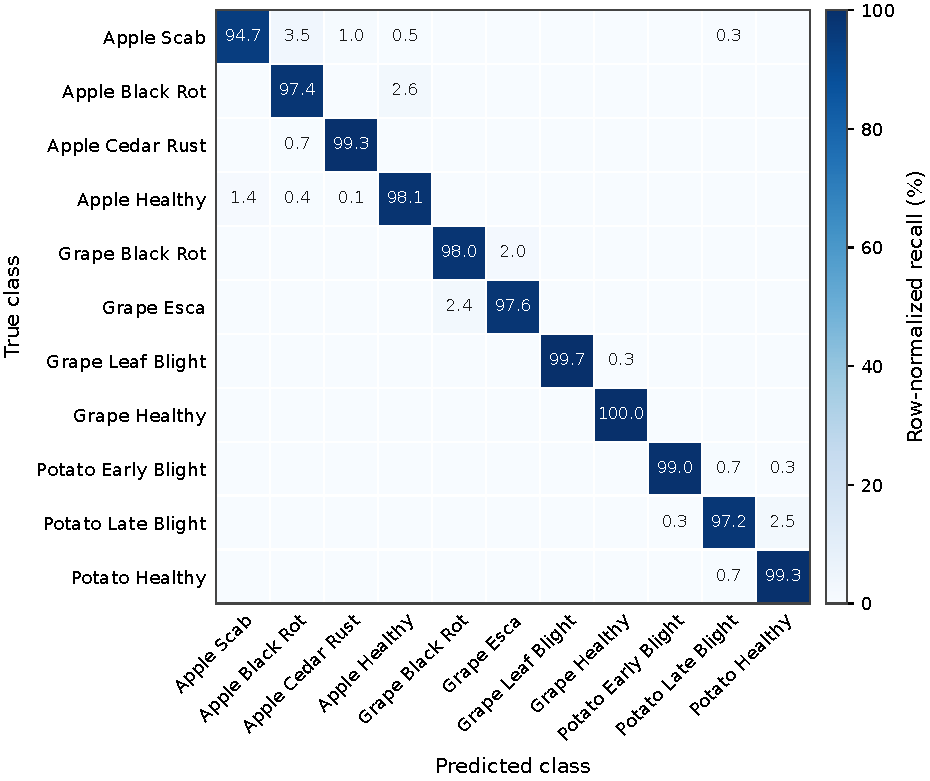
\includegraphics[width=0.82\columnwidth]{fig_confusion.pdf}
\caption{Row-normalized confusion matrix for BioDINO-Edge under transductive inference on the canonical PlantVillage split (9,330 test queries; 11 classes across Apple, Grape, and Potato). Rows represent ground-truth annotations; columns represent predictions. Diagonal entries indicate per-class recall (\%). Residual misclassifications concentrate strictly among pathologies of the same host species; cross-species confusion is negligible (0.021\%).}
\label{fig:confusion}
\end{figure}

\textbf{Engineering analysis of diagnostic errors and epidemiological safety.} As shown in Fig.~\ref{fig:confusion} and Table~\ref{tab:per_class}, classification errors are strictly confined within the same botanical host species. Residual confusion occurs primarily between Apple Scab and Apple Black Rot (F1 0.955 and 0.962), where early necrotic spots share visual circularity and chlorotic borders, as well as between intermediate symptom stages of Grape Esca and Black Rot (F1 0.979 and 0.976). Crucially for disease containment, cross-species confusion is near-zero: across 9,330 queries, only two apple scab leaves were erroneously attributed to potato late blight (a 0.021\% error rate). Furthermore, the framework achieves an exceptionally low false-negative rate (FNR) of 0.702\%, misclassifying only 50 out of 7,125 diseased leaves as healthy. Potato Healthy shows high recall (0.993) paired with moderate precision (0.839) under high class imbalance (147 healthy vs.\ $\approx$2,000 infected leaves), providing a safe, conservative triage strategy that prioritizes early pathogen containment.
